

\documentclass{beamer}


\usetheme{Madrid}

\usepackage[linesnumbered,ruled,vlined]{algorithm2e}
\usepackage{subcaption}
\usepackage{multirow}
\usepackage{booktabs}
\usepackage{threeparttable}
\usepackage{pbox}
\usepackage{ragged2e}
%\usepackage{subfig}
\usepackage{graphicx}
\usepackage{color}
\usepackage{float}
%\usepackage{algorithmic, algorithm2e, float}
\usepackage[absolute,overlay]{textpos}
\usepackage{pbox}
\usepackage{listings}
\usepackage{amsmath}
\usepackage{adjustbox}
\SetAlFnt{\small}
\SetAlCapFnt{\small}
\SetAlCapNameFnt{\small}
\setbeamertemplate{caption}[numbered]

\title[Open Seminar]{Intelligent Transportation Systems }


\subtitle{Algorithms and Formal Verification}

\author[A.P. Chouhan]{\textbf{Aaditya~Prakash~Chouhan}\\~\\ Supervised by: \textbf{Dr. Gourinath~Banda}}
% - Give the names in the same order as the appear in the paper.
% - Use the \inst{?} command only if the authors have different
%   affiliation.

\institute[IIT Indore] % (optional, but mostly needed)
{
Discipline of Computer Science and Engineering\\	
\textbf{Indian Institute of Technology Indore}\\~\\
\textit{phd1501201006@iiti.ac.in}

}
% - Use the \inst command only if there are several affiliations.
% - Keep it simple, no one is interested in your street address.

\date[October 8, 2020]{October 8, 2020}
% - Either use conference name or its abbreviation.
% - Not really informative to the audience, more for people (including
%   yourself) who are reading the slides online

% \subject{Uppaal verification of AIM}
% This is only inserted into the PDF information catalog. Can be left
% out. 

% If you have a file called "university-logo-filename.xxx", where xxx
% is a graphic format that can be processed by latex or pdflatex,
% resp., then you can add a logo as follows:

% \pgfdeclareimage[height=0.5cm]{university-logo}{university-logo-filename}
% \logo{\pgfuseimage{university-logo}}

% Delete this, if you do not want the table of contents to pop up at
% the beginning of each subsection:

% Un-comment these lines to show section layout after every subsection
% \AtBeginSubsection[]
% {
%   \begin{frame}<beamer>{Outline}
%     \tableofcontents[currentsection,currentsubsection]
%   \end{frame}
% }

% Let's get started
\begin{document}

\begin{frame}
  \titlepage
\end{frame}

\begin{frame}{Outline}
  \tableofcontents
  % You might wish to add the option [pausesections]
\end{frame}

% Section and subsections will appear in the presentation overview
% and table of contents.

\section{Intelligent Transportation Systems}
\subsection{Introduction and Motivation}
%\subsubsection{Autonomous Vehicles}
\begin{frame}{Intelligent Transportation Systems (ITS)}
The main objective of ITS is to use the technology present to our advantage. It involves managing the transportation network using real-time information for applications such as:
\begin{itemize}
	\item Traffic light management;
	\item Vehicle navigation;
	\item Emergency vehicle notification;
	\item Collision avoidance systems, etc.\\~\\
\end{itemize}
Advancements in the sensing, wireless communication and computational technologies has led to the development of various ITS applications.\\~\\
The induction of autonomous vehicles in transportation system will give rise to various new ITS applications.

\end{frame}

%\begin{frame}{Intelligent Transportation System}
%	The following figure shows a generalized architecture for an ITS.
%	
%\end{frame}

\begin{frame}{Autonomous Vehicle}
	An Autonomous Vehicle (AV) has an autonomous driver agent for the lateral and/or longitudinal control of the vehicle in some or all driving modes and conditions.\\~\\
	An AV makes use of various sensors for perception of the environment and localization. Lidar, Radar, Sonar, Camera, GPS, IMU (Inertial Measurement Unit), etc. are examples of AV sensors.
	\begin{figure}
		\centering
		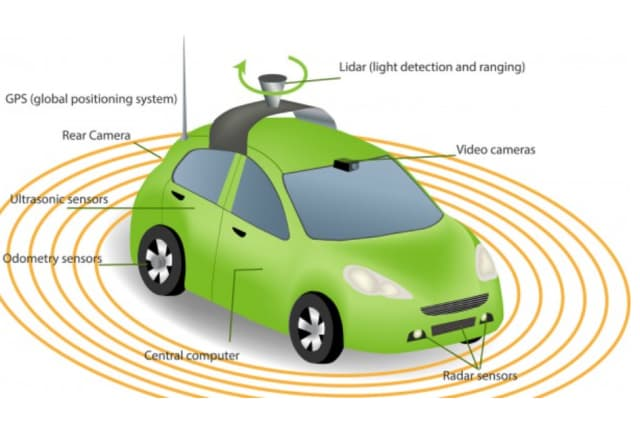
\includegraphics[scale = 0.25]{figures/AV sensors image coutsey_engineering}
		\caption{Sensors used in an AV}
		\label{avsensors}
	\end{figure}
\end{frame}
\begin{frame}{Autonomy Levels of AV}
	The level of autonomy an AV possess depends on:
	\begin{itemize} 
		\item Autonomous control over lateral and/or longitudinal movement,
		\item Who performs the object and event detection and response functionality
		\item The operational design domain of the vehicle\\~\\
		\end{itemize}
	Based on the above mentioned factors, 6 levels of autonomy are defined by the Socitey of Automotive Engineers (SAE) \footnotemark
	\footnotetext{SAE J3016: \textit{Levels of Driving Automation}}
\end{frame}

\begin{frame}{SAE Autonomy Levels}
	\begin{figure}
		\centering
		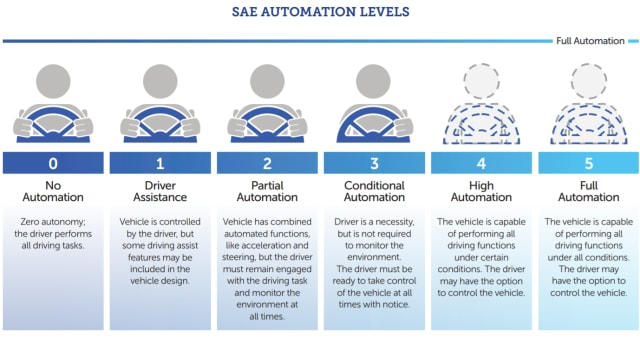
\includegraphics[width = \textwidth]{figures/SAE levels image coutsey_SAE}
		\caption{SAE autonomy levels (\textit{image courtesy of SAE})}
		\label{saelevels}
	\end{figure}
\end{frame}

\begin{frame}{ITS for AV}
	The induction of AV in transportation system will give rise to whole new possibilities of ITS algorithms.\\~\\
	Along with the freedom AV offers to human drivers, it is expected to have a huge impact on today's traffic management system as well. \\~\\
	Qualities of an AV that makes it useful for ITS applications are:
	\begin{itemize}
		\item Obedience
		\item Precision
		\item Highly cooperative
		\item Less unpredictable
	\end{itemize}
\end{frame}


\begin{frame}s
	\begin{center}
		\Huge Thank You!
	\end{center}
\end{frame}



\end{document}
